In \secref{prior_perturbations} we considered a multiplicative perturbations
of the form \eqref{phi_perturbation} with the $\norminf{\cdot}$ norm.  In
this section we consider other norms, illustrating that other choices
have problems with KL divergence.

First, we recall what we hope to get from our linear approximation.  We wish to
approximation $\etaopt(\phi)$ using the linear approximation $\etalin(\phi)$
evaluated at $\phiz$, hoping that the error $\norm{\etaopt(\phi) -
\etalin(\phi)}_2$ is small whenever the $\norm{\phi}$ is small (for some choice
of $\norm{\cdot}$).  A bare minimum for such a local approximation to work is
for $\phi \mapsto \etaopt(\phi)$ to be continuous, so that, for any
$\phi$,
%
\begin{align*}
%
\lim_{t \rightarrow 0} \norm{\etaopt(t \phi) - \etaopt}_2 = 0.
%
\end{align*}
%
By this reasoning, however, $\etaopt$ itself is a ``good'' approximation to
$\etaopt(\phi)$ when $\norm{\phi}$ is small---when $\phi$ is small, by
continuity we can simply say that nothing has changed and be reasonably correct.
From our linear approximation, we expect another order of accuracy, namely that
%
\begin{align*}
%
\lim_{t \rightarrow 0} \frac{\norm{\etaopt(t \phi) - \etalin(t\phi)}_2}{t} = 0.
%
\end{align*}

The preceding display is enough if we have a fixed $\phi$ in mind.  However, if
we want to search over a larger set of candidate $\phi$, we want the derivative
to provide a {\em uniformly good approximation} to $\etaopt(\phi)$ amonst some
set of $\phi$, say, all bounded $\phi: \norm{\phi} \le 1$.  One way of
formalizing the notion of ``uniformaly good approximation'' follows.

%%%%%%%%%%%%%%%%%%%%%%%%%%%%%%%%%%%%%%%%%%%%%%%%%%%%%%%%%%%%%%%%%%%%%%%%%%%
%%%%%%%%%%%%%%%%%%%%%%%%%%%%%%%%%%%%%%%%%%%%%%%%%%%%%%%%%%%%%%%%%%%%%%%%%%%
\begin{defn}\deflabel{diffable_classes}
    (\citep[Definition 4.5]{zeidler:2013:functional})
%
Let $B_1$ and $B_2$ denote Banach spaces, and let $\ball_1 \subseteq B_1$ define
an open neighborhood of $\phi_0 \in B_1$.  Fix a function $f: \ball_1
\mapsto B_2$.

The function $f$ is {\em directionally differentiable} (also known as a Gateaux
differentiable) if there exists a bounded linear functional $f^{\mathrm{lin}}:
B_1 \mapsto B_2$ such that the following condition holds for any
$\phi$ with $\norm{\phi - \phi_0} < \infty$:
%
\begin{align*}
%
%\textrm{For any }\phi\textrm{ with }\norm{\phi - \phi_0} < \infty\textrm{, }
\lim_{t \rightarrow 0}
    \frac{f(\phi) - f(\phi_0) -
          f^{\mathrm{lin}}(t (\phi - \phi_0) )
         }{t} \rightarrow 0.
%
\end{align*}
%

Similarly, the function $f$ is {\em boundedly differentiable} (also known as
Fr{\'echet} differentiable) at $\phi_0$ if we can take the limit uniformly in
$\phi$:
%
\begin{align*}
%
\lim_{t \rightarrow 0}
    \sup_{\phi: \norm{\phi - \phi_0} = 1}
    \frac{f(\phi) - f(\phi_0) -
          f^{\mathrm{lin}}(t (\phi - \phi_0))
         }{t} \rightarrow 0.
%
\end{align*}
%
\end{defn}
%%%%%%%%%%%%%%%%%%%%%%%%%%%%%%%%%%%%%%%%%%%%%%%%%%%%%%%%%%%%%%%%%%%%%%%%%%%

Note that we used the same notation $f^{\mathrm{lin}}$ for both derivatives in
\defref{diffable_classes}.  In fact, if a function is compactly differentiable
then the two derivatives must coincide \citep[Proposition
4.8]{zeidler:2013:functional}, which justifies our presumptuous notation.

% The difference between bounded and directional differentiability is whether the
% linear approximation holds uniformly in $\phi$.

It is possible for functions to be directionally but not boundedly
differentiable even in $\mathbb{R}^2$, as the following example demonstrates.

%%%%%%%%%%%%%%%%%%%%%%%%%%%%%%%%%%%%%%%%%%%%%%%%%%%%%%%%%%%%%%%%%%%%%%%%%
%%%%%%%%%%%%%%%%%%%%%%%%%%%%%%%%%%%%%%%%%%%%%%%%%%%%%%%%%%%%%%%%%%%%%%%%%
\begin{ex}\exlabel{r2_pathological}
%
Consider $(x_1, x_2) \in \mathbb{R}^2$ and the polar coordinates $r :=
\sqrt{x_1^2 + x_2^2}$ and $\theta := \arctan(x_2 / x_1)$.  Let $\{\pi k: k \in
\mathbb{Z} \}$ denote integer multiples of $\pi$.  Define
%
% \begin{align*}
% %
% f(r, \theta) := \begin{cases}
% \frac{\left(\frac{r}{| \sin \theta |}\right)^2}
%      {1 + \left(\frac{r}{| \sin \theta |}\right)^2}
%     & \textrm{when } \theta \notin \{\pi k: k \in \mathbb{Z}\}
%     \textrm{ and } r > 0 \\
% 0. & \textrm{when } \theta \in \{\pi k: k \in \mathbb{Z}
%     \} \textrm{ or }r = 0
% %
% \end{cases}
\begin{align*}
%
f(r, \theta) := \begin{cases}
    \left(\frac{r}{| \sin \theta |}\right)^2
        & \textrm{when } \theta \notin \{\pi k: k \in \mathbb{Z}\}
        \textrm{ and } r > 0 \\
    0. & \textrm{when } \theta \in \{\pi k: k \in \mathbb{Z}
        \} \textrm{ or }r = 0
%
\end{cases}
%
\end{align*}
%
%%%%%%%%%%%%%%%%%%%%%%%%%%%%%%%%%%%%%%%%%%%%%%%%%%%%%%%%%%%%%%%%%%%%%%%%%
%%%%%%%%%%%%%%%%%%%%%%%%%%%%%%%%%%%%%%%%%%%%%%%%%%%%%%%%%%%%%%%%%%%%%%%%%
\begin{figure}[h!]

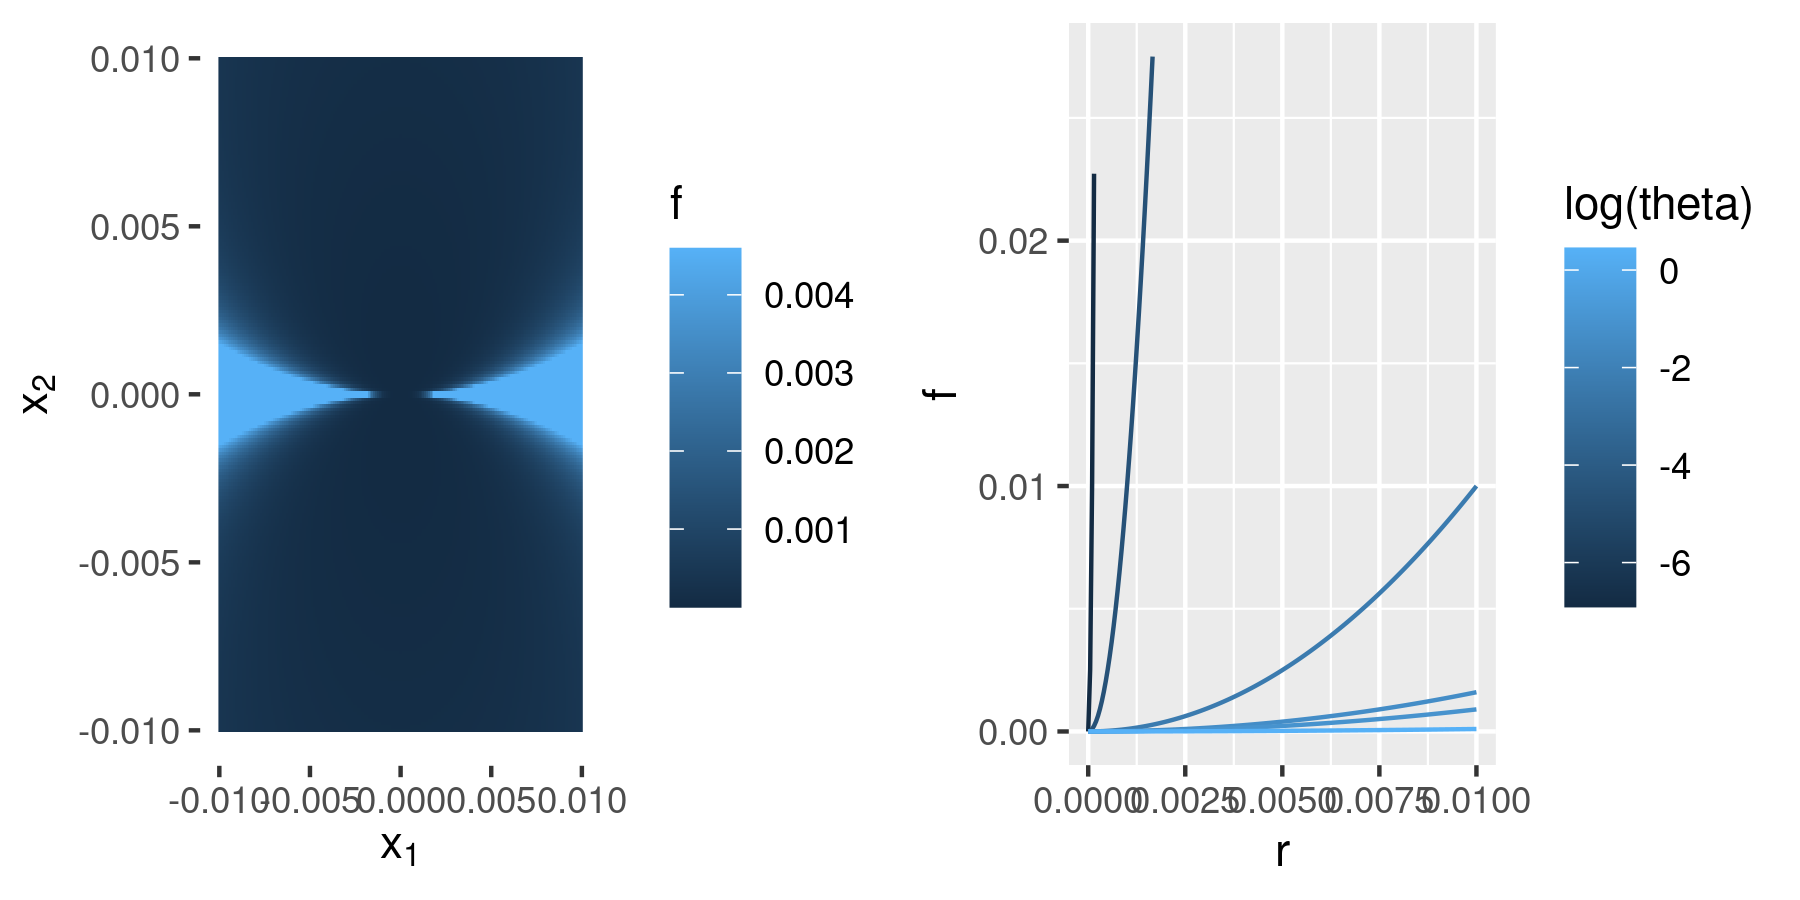
\includegraphics[width=0.980\linewidth,height=0.490\linewidth]{static_images/pathological_r2_example.png}
\caption{A plot of $f(x_1, x_2)$ from \exref{r2_pathological}.}
\figlabel{r2_pathological}
\centering
\end{figure}
%%%%%%%%%%%%%%%%%%%%%%%%%%%%%%%%%%%%%%%%%%%%%%%%%%%%%%%%%%%%%%%%%%%%%%%%%
%
\Figref{r2_pathological} contains a plot of $f(r, \theta)$, both over
$\mathbb{R}^2$ and along paths for particular choices of $\theta$.

Then $f$ has a directional derivative in every direction, but is not Fr{\'e}chet
differentiable.  By ordinary calculus, for any $\theta$, $\fracat{\partial f(r,
\theta)}{\partial r}{r=0} = 0$, so the directional derivatives all exist and are
identically $0$.  However, for any $r$, there exists a $\theta(r)$ such that $r /
|\sin(\theta(r))| = 1$.  For such a choice of $\theta(r)$, the error in the
linear approximation is $f(r, \theta(r)) - 0 = 1/2$, which does not go to zero
as $r \rightarrow 0$.

\end{ex}
%%%%%%%%%%%%%%%%%%%%%%%%%%%%%%%%%%%%%%%%%%%%%%%%%%%%%%%%%%%%%%%%%%%%%%%%%

Note that the second derivative in a particular direction is given by
$\fracat{\partial^2 f(r, \theta)}{\partial r^2}{r=0} = \frac{1}{2 |\sin
\theta|}$, which can be made arbitrarily large by taking $\theta$ close to $0$
or to $\pi$.  We could modify $f(r, \theta)$ to be Fr{\'e}chet differentiable
by smoothly ``capping'' $1 / |\sin \theta|$ at some arbitrarily large value.
However, the ability to meaningfully extrapolate $f(r, \theta)$ in the direction
of a very large but finite second derivative will still be extremely limited. In
this sense, Fr{\'e}chet differentiability is a weak necessary but not sufficient
requirement if we are interested in extrapolating using linear approximations.



%%%%%%%%%%%%%%%%%%%%%%%%%%%%%%%%%%%%%%%%%%%%%%%%%%%%%%%%%%%%%%%%%%%%%%%%%
%%%%%%%%%%%%%%%%%%%%%%%%%%%%%%%%%%%%%%%%%%%%%%%%%%%%%%%%%%%%%%%%%%%%%%%%%
\begin{ex}\exlabel{r2_pathological_v2}
%
In the context of \exref{r2_pathological}, fix some $0 < M < \infty$,
and define
%
\begin{align*}
%
\tilde{f}(r, \theta) := \begin{cases}
    f(r, \theta) & \textrm{when }\frac{1}{\abs{\sin(\theta)}} \le M \\
    0. & \textrm{when }\frac{1}{\abs{\sin(\theta)}} > M.
%
\end{cases}
%
\end{align*}
%
Then $\tilde{f}$ is continuous and Fr{\'e}chet differentiable at $r=0$. In this
case, for any $r$, $\sup_{\theta} r / |\sin(\theta(r))| = r / M$, so  both
$\lim_{r \rightarrow 0} \tilde{f}(r, \theta) \le \lim_{r \rightarrow 0} r^2 /
M^2 = 0$ and $\lim_{r \rightarrow 0} \tilde{f}(r, \theta) / r \le \lim_{r
\rightarrow 0}  r / M^2 = 0$.  (Note that $\tilde{f}$ is continuous only
at $r=0$, not on a ball centered at $0$.)

Despite being Fr{\'e}chet differentiable, the linear approximation may not
extrapolate well to any finite $r$.  In the direction $\theta = \sin^{-1}(1 /
M)$, the error of the linear extrapolation to any $r_0$ is still $\tilde{f}(r,
\theta) - 0 = M r_0^2$. Since Fr{\'e}chet differentiability requires only $M <
\infty$, the extraplation error can be arbitrarily large, even for Fr{\'e}chet
differentiable functions.

\end{ex}
%%%%%%%%%%%%%%%%%%%%%%%%%%%%%%%%%%%%%%%%%%%%%%%%%%%%%%%%%%%%%%%%%%%%%%%%%


\Exref{r2_pathological} is neither Fr{\'e}chet differentiable nor continuous,
whereas \exref{r2_pathological} is both Fr{\'e}chet differentiable and
continuous.  In general, however, Fr{\'e}chet differentiability is stronger than
continuity, in the sense that Fr{\'e}chet differentiability implies continuity,
but continuity does not imply Fr{\'e}chet differentiability \citep[Proposition
4.8 (d)]{zeidler:2013:functional}.  See also \citet[Example
1.9]{averbukh:1967:theory} for a simple example of a function on $\mathbb{R}^2$
that is continuous and directionally differentiable but not Fr{\'e}chet
differentiable.

The sort of pathology exhibited by \exref{r2_pathological, r2_pathological_v2}
requires some care to construct in $\mathbb{R}^2$, but requires some care to
avoid in infinite-dimensional spaces.  We now give an illustrative example in
the $\lp{p}$ spaces; since the result will be important for VB prior
sensitivity, we will state is as a lemma rather than merely an example.

%%%%%%%%%%%%%%%%%%%%%%%%%%%%%%%%%%%%%%%%%%%%%%%%%%%%%%%%%%%%%%%%%%%%%%%%%
%%%%%%%%%%%%%%%%%%%%%%%%%%%%%%%%%%%%%%%%%%%%%%%%%%%%%%%%%%%%%%%%%%%%%%%%%
\begin{lem}\lemlabel{e_log_nonfrechet}

% TODO: make this a lemma.  Then, by saying that \assuref{dist_fun_nice}
% holds with $\int M_\psi(\zeta)^{1/q} d\zeta < \infty$ for $1 \le q < \infty$,
% I think you will get existence of the $L_p$ derivatives.

Fix $1 \le p < \infty$, and let $q = (1 - p^{-1})^{-1}$, from which $p^{-1} +
q^{-1}=1$ follows.\footnote{Regrettably the standard choices of $p$ and $q$ for
$\lp{p}$ spaces and their duals overlap with our notation for probability and
variational distributions, but there should be no ambiguity in context.}  Let
$\q(\zeta)$ be a density relative to the Lebesgue measure on $[0,1]$ such that
$\int \q(\zeta)^q d\zeta < \infty$. Define $f: \lp{p} \mapsto \mathbb{R}$ as
follows:
%
\begin{align*}
%
f(\phi) :=
\begin{cases}
    %
    \expect{\q(\zeta)}{\log \left(1 + \phi(\zeta)\right)} &
    \textrm{when }\phi(\zeta) > -1\textrm{ almost surely} \\
    %
    0 & \textrm{otherwise}.
%
\end{cases}
%
\end{align*}
%
Then $f$ is discontinous at $\phiz$ in $\norm{\cdot}_p$ and so not Fr{\'e}chet
differentiable.  However $f$ has a directional derivative at $\phiz$ in every
direction $\phi - \phiz$.

\begin{proof}
%
For any $0 < \epsilon < 1$, let $S_\epsilon \subset [0, 1]$ be a measurable set
with Lebesgue measure $\epsilon$ and probability at least $\epsilon$ under
$\q(\zeta)$.  Such a set must exist because $\int_0^1 \q(\zeta) d\zeta = 1$. For
$\delta > 0$ let
%
\begin{align*}
%
\phi(\zeta; \epsilon, \delta) :=
\begin{cases}
    %
    \delta - 1      & \textrm{ for }\zeta\in S_\epsilon \\
    0      & \textrm{ for }\zeta\notin S_\epsilon.
    %
\end{cases}
%
\end{align*}
%
Then $\phi(\zeta; \epsilon, \delta) \in \lp{p}$ with $\norm{\phi(\cdot;
\epsilon, \delta)}_p = (\int_0^1 \phi(\zeta)^p d\zeta)^{1/p} =\epsilon^{1/p}
(\delta - 1)$.  Furthermore,
%
\begin{align*}
%
\abs{f(\phi(\zeta; \epsilon, \delta))} ={}&
    \expect{\q(\zeta)}{\ind{\zeta \in S_\epsilon}} \abs{\log(\delta)} \ge
    \epsilon \abs{\log(\delta)}.
%
\end{align*}
%,
Take $\delta(\epsilon) = \exp(-\epsilon)$.  Then, for any sequence $\epsilon_n
\rightarrow 0$,
%
\begin{align*}
%
\abs{f(\phi(\zeta; \epsilon_n, \delta(\epsilon_n))) - f(\phiz)} \ge{} 1
\mathtxt{and}
\norm{\phi(\cdot; \epsilon_n, \delta(\epsilon_n))}_p \rightarrow{} 0.
%
\end{align*}
%
So $f$ is discontinuous on an $\norm{\cdot}_p$ ball containing $\phiz$, and
cannot be Fr{\'e}chet differentiable.

However, the directional derivative exists in any direction. First, suppose that
$\inf_{\zeta} \phi(\zeta) = -\infty$.  Then $\inf_{\zeta} t \phi(\zeta) =
-\infty$ for any $t > 0$, so $f(t\phi) = 0$ for all $t$, and $\lim_{t
\rightarrow 0} (f(t \phi) - f(\phiz)) / t = \lim_{t \rightarrow 0} 0 = 0$.

If $-\infty < \inf_\zeta \phi(\zeta)$, then there exists a $t_0 > 0$ such that
$t_0 \phi(\zeta)$ is strictly larger than $-1$.  Let us consider only $t < t_0$.
If we can apply the dominated convergence theorem, then
%
\begin{align*}
%
\fracat{\partial f(t \phi)}{\partial t}{t=0} ={}&
    \int \q(\zeta) \fracat{\partial \log(1 + t \phi(\zeta))}{\partial t}{t=0} d\zeta
\\={}&
\int \q(\zeta) \phi(\zeta) d\zeta.
%
\end{align*}
%
The directional derivative in the direction $\phi - \phiz$ at $\phiz$ would thus
be given by $\expect{\q(\zeta)}{\phi(\zeta)}$.

If $\sup_\zeta \phi(\zeta) < \infty$ then we can apply the dominated convergence
theorem with a multiple of the constant function.  For the case $\sup_\zeta
\phi(\zeta) = \infty$, observe that
%
\begin{align*}
%
f(\phi) ={}&
    \int \q(\zeta) \log(1 + \phi(\zeta)) \ind{\phi(\zeta) \le 0} d\zeta + \\
    &\int \q(\zeta) \log(1 + \phi(\zeta)) \ind{\phi(\zeta) > 0} d\zeta.
%
\end{align*}
%
The integrand $\log(1 + \phi(\zeta)) \ind{\zeta \le 0}$ of the first term
is bounded, so we can apply the DCT.  For the second term,
%
\begin{align*}
%
\q(\zeta) \log(1 + t \phi(\zeta)) \ind{t \phi(\zeta) > 0}   \le{}&
    \q(\zeta) (1 + t \phi(\zeta)) \ind{t \phi(\zeta) > 0}.%
\end{align*}
%
Without loss of generality we can take $t < 1$ so that the preceding display is
integrable for all $t$ whenever $\int \q(\zeta) \abs{\phi(\zeta)} d\zeta <
\infty$. But this follows by Holder's inequality with the Lebesgue measure,
since
%
\begin{align*}
%
\int_0^1 \q(\zeta) \abs{\phi(\zeta)} d \zeta \le{}&
    \left( \int \q(\zeta)^q d\zeta \right)^{1/q}
    \left( \int \abs{\phi(\zeta)}^p d\zeta \right)^{1/p} \le \infty.
%
\end{align*}
%
%
\end{proof}
%
\end{lem}
%%%%%%%%%%%%%%%%%%%%%%%%%%%%%%%%%%%%%%%%%%%%%%%%%%%%%%%%%%%%%%%%%%%%%%%%%


We can define the family of nonlinear perturbations similar to
\citep{gustafson:1996:local}.

%%%%%%%%%%%%%%%%%%%%%%%%%%%%%%%%%%%%%%%%%%%%%%%%%%%%%%%%%%%%%%%%%%%%%%%%%
%%%%%%%%%%%%%%%%%%%%%%%%%%%%%%%%%%%%%%%%%%%%%%%%%%%%%%%%%%%%%%%%%%%%%%%%%
\begin{defn}\deflabel{prior_nl_pert}
%
Fix $\pbase(\nu)$ and $1 \le p \le \infty$.  For any $\phi \in \lp{p}$, define
\footnote{We have dropped a factor of $p$ from the perturbation when $p <
\infty$ relative to the definition in \citep{gustafson:1996:local}.}
%
\begin{align*}
%
\pstick'(\nu \vert \phi) :={}& \begin{cases}
%
\left(\pbase(\nu)^{-1} + \phi(\nu) \right)^{p}
    & \textrm{when }p < \infty \\
\pbase(\nu)\exp(\phi(\nu))
    & \textrm{when }p = \infty
%
\end{cases}\\
%
\pstick(\nu \vert \phi) :={}&
    \frac{\pstick'(\nu \vert \phi)}{\int \pstick'(\nu' \vert \phi) d\nu'}.
%
\end{align*}
%
\end{defn}
%
%%%%%%%%%%%%%%%%%%%%%%%%%%%%%%%%%%%%%%%%%%%%%%%%%%%%%%%%%%%%%%%%%%%%%%%%%

\Defref{prior_nl_pert} provides one class of answers to what it means to perturb
a prior, and how to measure the size of the perturbation.  \citep[Result
2]{gustafson:1996:local} states that using $\norm{\cdot}_p$ with its
corresponding perturbation gives a notion of ``size'' of a perturbation that is
a norm, invariant to changes in the base measure, and invariant under one-to-one
re-parameterizations.

Unlike \citep{gustafson:1996:local}, we allow the perturbations $\phi$ to be
negative.  There are two reasons for doing so.  First, if $\phi$ must be
pointwise positive, then $\pstick(\nu \vert \phi)$ is not defined in an open
ball containing $\phiz$, and standard results from functional analysis cannot be
directly applied to establish properties like Fr{\'e}chet differentiability.
There may be priors that cannot be achieved by considering only positive
perturbations.  But perhaps most importantly, when $\phi$ must be positive, the
norm $\norm{\cdot}_p$ treats ablating and adding prior mass very asymmetrically
when $p < \infty$, arguably violating an intutive notions of the ``size''
of perturbation.

Suppose $p < \infty$ and we wish to choose a $\phi$ to change $\pbase$ into
$\palt$, for which \defref{prior_nl_pert} gives that we must choose
%
\begin{align}\eqlabel{phi_for_palt}
%
\phi(\nu) = \alpha \palt(\nu)^{1/p} - \pbase(\nu)^{1/p}
    \mathtxt{where}\alpha > 0.
%
\end{align}
%
The fact that we are free to choose $\alpha$ follows from the fact that we
normalize after perturbing.  As long as $\palt(\nu) > 0$ whenever $\pbase(\nu) >
0$ (a condition which is certainly not always satisfied), one can choose
%
\begin{align*}
%
\alpha = \sup_{\nu} \left(\frac{\pbase(\nu)}{\palt(\nu)}\right)^{1/p}
%
\end{align*}
%
to guarantee that $\phi(\nu)$ is non-negative.  However, by doing so, one might
have to create a ``large'' perturbation, according to the $\norm{\cdot}_p$,
as the following \exref{positive_pert_large} demonstrates.

% %%%%%%%%%%%%%%%%%%%%%%%%%%%%%%%%%%%%%%%%%%%%%%%%%%%%%%%%%%%%%%%%%%%%%%%%%
% \begin{ex}
% %
% Let $\pbase(\nu) = \frac{4}{3}\ind{\frac{1}{4} \le \nu \le 1}$ and $\palt(\nu) =
% \frac{4}{3}\ind{0 \le \nu \le \frac{3}{4}}$.  Then, for any $\alpha > 0$, any $1
% \le p < \infty$, and for $\phi$ as given in \eqref{phi_for_palt}, $\phi(7/8) <
% 0$.  So there is no value of $\alpha$ that can transform $\pbase$ into $\palt$
% using only a positive perturbation.
% %
% \end{ex}
%%%%%%%%%%%%%%%%%%%%%%%%%%%%%%%%%%%%%%%%%%%%%%%%%%%%%%%%%%%%%%%%%%%%%%%%%
%%%%%%%%%%%%%%%%%%%%%%%%%%%%%%%%%%%%%%%%%%%%%%%%%%%%%%%%%%%%%%%%%%%%%%%%%


%%%%%%%%%%%%%%%%%%%%%%%%%%%%%%%%%%%%%%%%%%%%%%%%%%%%%%%%%%%%%%%%%%%%%%%%%
\begin{ex}\exlabel{positive_pert_large}
%

%%%%%%%%%%%%%%%%%%%%%%%%%%%%%%%%%%%%%%%%%%%%%%%%%%%%%%%%%%%%%%%%%%%%%%%%%
%%%%%%%%%%%%%%%%%%%%%%%%%%%%%%%%%%%%%%%%%%%%%%%%%%%%%%%%%%%%%%%%%%%%%%%%%
\begin{figure}[h!]

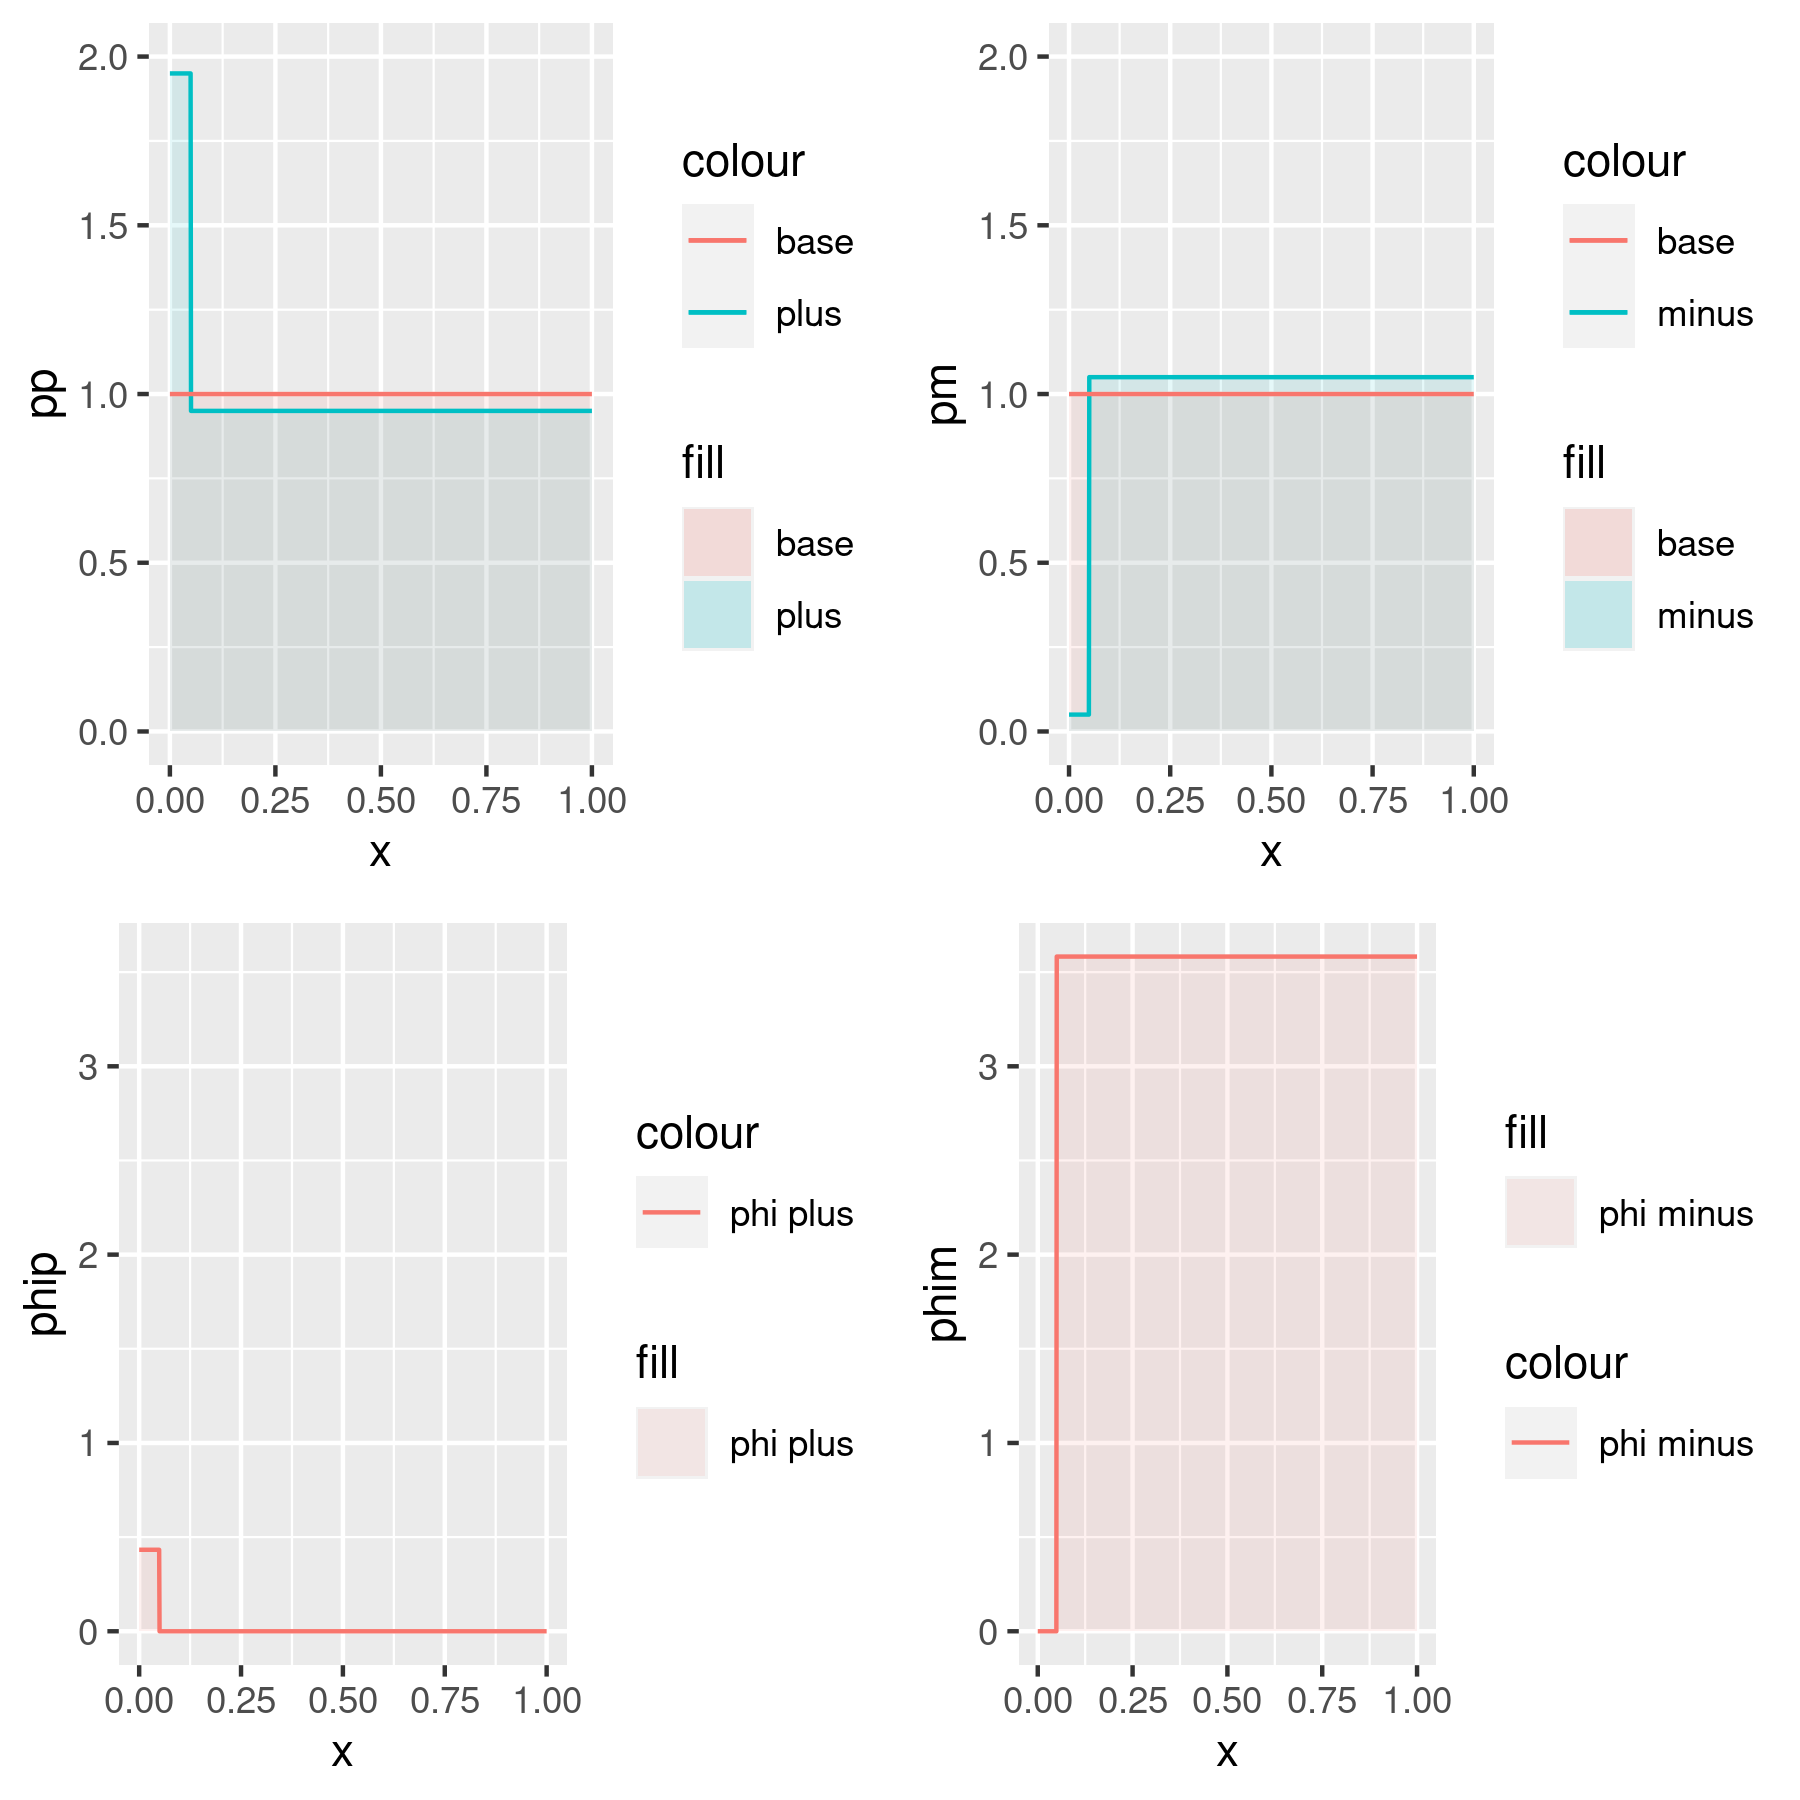
\includegraphics[width=0.980\linewidth,height=0.980\linewidth]{static_images/positive_phi_example.png}
%
\caption{A plot of the perturbations from \exref{positive_pert_large}
with $p=2$ and $\epsilon=0.05$.  Positive $\phi$ can only add mass, so to remove
a small amount of mass requires adding mass everywhere else and re-normalizing,
resulting in a large perturbation according to $\norm{\cdot}_p$.}
%
\figlabel{positive_pert_large}
\centering
\end{figure}
%%%%%%%%%%%%%%%%%%%%%%%%%%%%%%%%%%%%%%%%%%%%%%%%%%%%%%%%%%%%%%%%%%%%%%%%%

Let $\pbase(\nu) = \ind{0 \le \nu \le 1}$.  For some $\delta > 0$ and $0 <
\epsilon \ll 1$, let
%
\begin{align*}
%
\palt(\nu) :={}&
    \left(\frac{1-\delta \epsilon}{1 - \epsilon} \right)
        \ind{\epsilon \le \nu \le 1} +
    \delta \ind{0 \le \nu \le \epsilon}.
% \\\approx{}&
%     \left(1-\delta \epsilon \right)
%         \ind{\epsilon \le \nu \le 1} +
%     \delta \ind{0 \le \nu \le \epsilon}
%
\end{align*}
%
% where the final approximation is due to the smallness of $\epsilon$.
Then \eqref{phi_for_palt} gives, for some $\alpha$,
%
\begin{align*}
%
\phi ={}&
    \left( \alpha\left(\frac{1-\delta \epsilon}{1-\epsilon} \right)^{1/p}
        - 1
    \right)
        \ind{\epsilon \le \nu \le 1} +
    \left(\alpha \delta^{1/p} - 1 \right) \ind{0 \le \nu \le \epsilon}.
%
% \\\approx{}&
%     \left( \alpha\left(1-\delta \epsilon \right)^{1/p}
%         - 1
%     \right)
%         \ind{\epsilon \le \nu \le 1} +
%     \left(\alpha \delta^{1/p} - 1 \right) \ind{0 \le \nu \le \epsilon}.
%
\end{align*}
%
And
%
\begin{align*}
%
\norm{\phi}_p ={}&
    \left( \alpha\left(\frac{1-\delta \epsilon}{1-\epsilon} \right)^{1/p} - 1
    \right) (1- \epsilon) +
    \left(\alpha \delta^{1/p} - 1 \right) \epsilon.
%
\end{align*}
%
For $\phi$ to be positive, we require
%
\begin{align*}
%
\alpha^p \ge \frac{1 - \epsilon}{1 - \delta \epsilon}
    \mathtxt{and}
\alpha^p \ge \frac{1}{\delta}.
%
\end{align*}

First, let us consider adding a small amount of prior mass, taking $\delta = 2 -
\epsilon$; let the corresponding perturbation be $\phi^+$.  For $\delta > 1$,
then we achieve $\phi \ge 0$ by taking $\alpha^p = \frac{1 - \epsilon}{1 -
\delta \epsilon}$.  Using the fact that $\epsilon \ll 1$ and keeping only
leading-order terms,
%
\begin{align*}
%
\frac{1-\epsilon}{1 - \delta \epsilon} \approx{}&
    (1- \epsilon)(1 + \delta \epsilon)
\\\approx{}& 1 + (\delta - 1) \epsilon
\\\approx{}& 1 + \epsilon,
%
\end{align*}
%
so
%
\begin{align*}
%
\norm{\phi^+}_p  ={}&
    \left(\alpha \delta^{1/p} - 1 \right) \epsilon
\\\approx{}&
    \left(
        \left( \left(1 + \epsilon\right) \left(2 - \epsilon \right)\right)^{1/p}
        - 1 \right) \epsilon
\\\approx{}&
%
\left( 2^{1/p} - 1 \right) \epsilon.
%
\end{align*}
%

Next, consider removing the same amount of mass with the symmetric change
$\delta = \epsilon$, letting $\phi^-$ be the corresponding perturbation. Then we
can ensure that $\phi(\nu) \ge 0$ with $\alpha^p \ge \epsilon^{-1}$, and
$\epsilon \ll 1$ gives
%
\begin{align*}
%
\frac{1-\delta\epsilon}{1 - \epsilon} \approx{}& 1- \epsilon,
%
\end{align*}
%
and
%
\begin{align*}
%
\norm{\phi^-}_p  ={}&
    \left( \alpha\left(\frac{1-\delta \epsilon}{1-\epsilon} \right)^{1/p} - 1
    \right) (1- \epsilon)
\\\approx{}&
\left(\left(\frac{1- \epsilon}{\epsilon}  \right)^{1/p} - 1\right)(1 - \epsilon)
%
\\\approx{}&
    \left( \frac{1}{\epsilon}\right)^{1/p}.
%
\end{align*}

Since $\epsilon$ is small, $\norm{\phi^-}_p \approx \left(
\frac{1}{\epsilon}\right)^{1/p} \gg \norm{\phi^+}_p \approx \left( 2^{1/p} - 1
\right) \epsilon$, despite the two perturbations respectively removing and
adding the same amount of arbitrarily small probability mass.

\end{ex}
%%%%%%%%%%%%%%%%%%%%%%%%%%%%%%%%%%%%%%%%%%%%%%%%%%%%%%%%%%%%%%%%%%%%%%%%%
%%%%%%%%%%%%%%%%%%%%%%%%%%%%%%%%%%%%%%%%%%%%%%%%%%%%%%%%%%%%%%%%%%%%%%%%%
